\documentclass[12pt, a4paper]{article}
\usepackage[francais]{babel}
\usepackage{caption}
\usepackage{graphicx}
\usepackage[T1]{fontenc}
\usepackage{listings}
\usepackage{geometry}
\usepackage[colorlinks=true,linkcolor=black,anchorcolor=black,citecolor=black,filecolor=black,menucolor=black,runcolor=black,urlcolor=black]{hyperref}

% \usepackage{mathpazo} --> Police à utiliser lors de rapports plus sérieux

\usepackage{fancyhdr}
\pagestyle{fancy}
\lhead{}
\rhead{}
\chead{}
\rfoot{\thepage}
\lfoot{Martin Baumgaertner}
\cfoot{}

\renewcommand{\headrulewidth}{0.4pt}
\renewcommand{\footrulewidth}{0.4pt}

\begin{document}
\begin{titlepage}
	\newcommand{\HRule}{\rule{\linewidth}{0.5mm}} 
	\center 
	\textsc{\LARGE iut de colmar}\\[6.5cm] 
	\textsc{\Large R4ROM19}\\[0.5cm] 
	\textsc{\large Année 2022-23}\\[0.5cm]
	\HRule\\[0.75cm]
	{\huge\bfseries TP 2 - Docker-compose}\\[0.4cm]
	\HRule\\[1.5cm]
	\textsc{\large martin baumgaertner}\\[6.5cm] 

	\vfill\vfill\vfill
	{\large\today} 
	\vfill
\end{titlepage}
\newpage
\tableofcontents
\newpage
\section{Déployer et gérer une stack de services interconnectés}
\subsection{Première configuration}
\subsubsection{Question 2-3-4}
Après avoir crée mon fichier yaml et l'avoir renseigné,
j'ai pu le lancer avec la commande \textbf{docker- compose -f docker-compose.yaml up -d}
Je peux très bien visualiser les composants démarrés avec \textbf{docker-compose ps}, 
je peux obtenir le même résultat que cette commande si je fais \textbf{docker ps -all}.
Voici donc ce que j'obtiens : 
\begin{figure}[h]
    \centering
    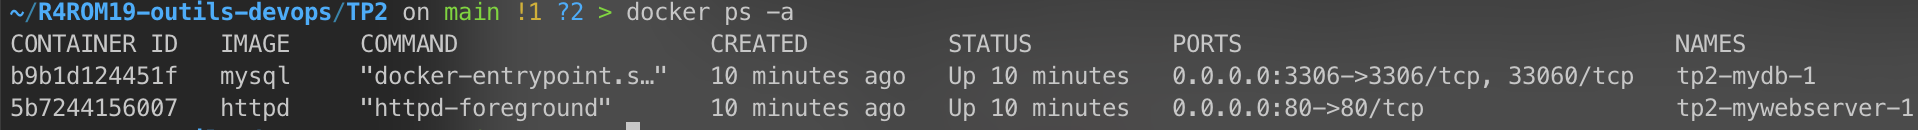
\includegraphics[width=1\textwidth]{img/ps-a.png}
    \caption{docker ps -all}
    \label{fig:ps-a}
\end{figure}\\

Je peux aussi bien entendu visualiser les logs avec \textbf{docker-compose logs}
\begin{figure}[h]
    \centering
    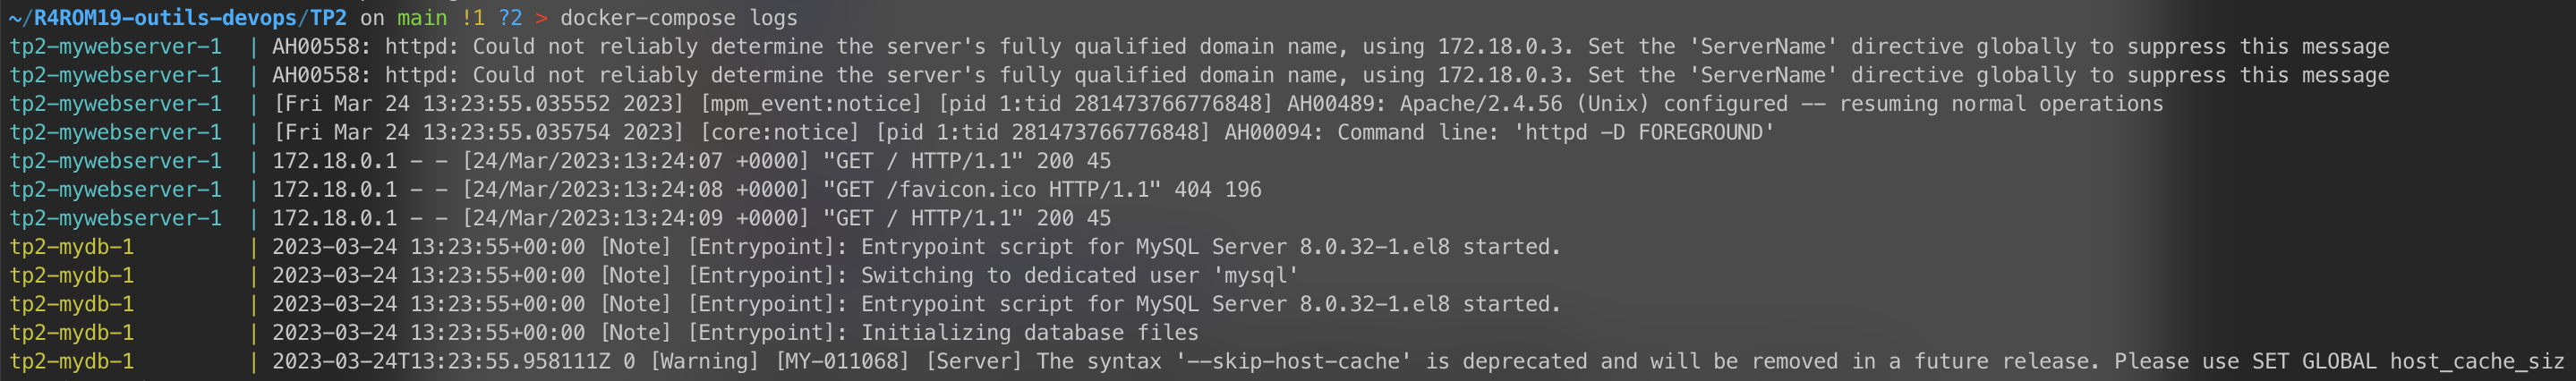
\includegraphics[width=1\textwidth]{img/logs.png}
    \caption{docker-compose logs}
    \label{fig:logs}
\end{figure}\\

\subsubsection{Question 5}
Je me connecte au docker avec la commande \textbf{docker exec -it tp2-mydb-1 /bin/bash}
On peut constater que j'atteris bien dans le docker en bash.
\begin{figure}[h]
    \centering
    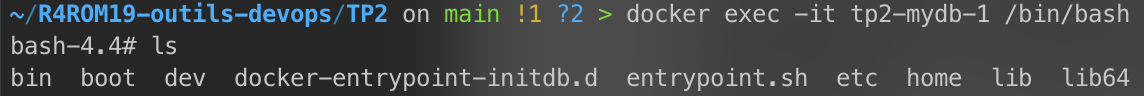
\includegraphics[width=1\textwidth]{img/connexion.png}
    \caption{Connexion à la base de données}
    \label{fig:connexion}
\end{figure}

\newpage
J'ai aussi bien évidemment accès la base de données en m'y connectant avec la commande \textbf{mysql -u root -p}
\begin{figure}[h]
    \centering
    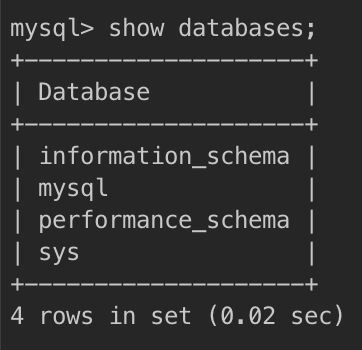
\includegraphics[width=0.4\textwidth]{img/bdd.png}
    \caption{Connexion à la base de données}
    \label{fig:bdd}
\end{figure}

\newpage
\subsection{Configuration de services interconnectés}
\subsubsection{Question 1-2}
Je viens donc modifier mon fichier de configuration du docker \textbf{docker-compose.yaml}.
de cette manière, pour y ajouter toutes les demandes de l'exercice.

\begin{figure}[h]
    \centering
    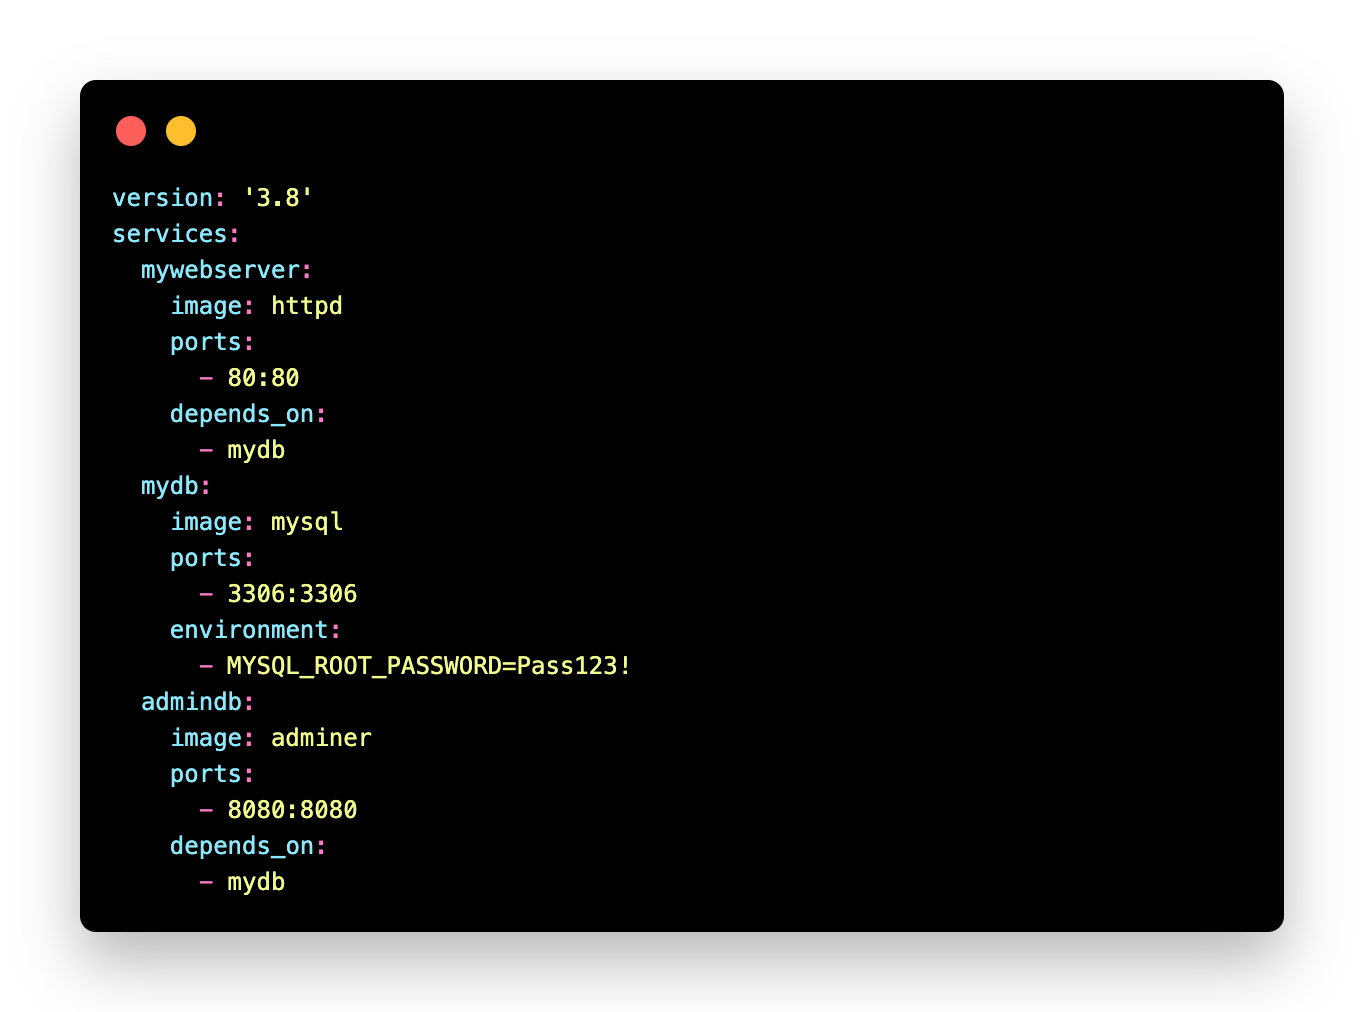
\includegraphics[width=1\textwidth]{img/code.png}
    \caption{docker-compose.yaml}
    \label{fig:code}
\end{figure}

\newpage
\section{Réaliser et publier son image Docker}
\subsection{Créer un fichier Dockerfile}
\subsubsection{Question a}
J'ai donc crée un fichier \textbf{Dockerfile} dans lequel j'ai renseigné les commandes suivantes :
\begin{lstlisting}
    FROM alpine
    ENTRYPOINT ["date"]
\end{lstlisting}

Puis, j'ai lancé la compilation avec \textbf{docker build -t afficher-date .}. Et 
pour finir je l'ai lancé avec \textbf{docker run -it afficher-date}. On peut bien évidemment
vérifier sa présence : \textbf{docker ps -a}.
\begin{figure}[h]
    \centering
    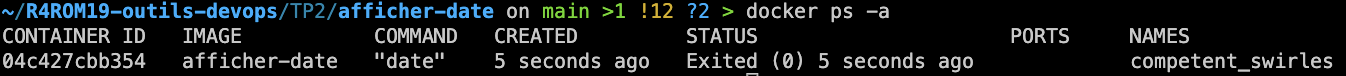
\includegraphics[width=1\textwidth]{img/psa.png}
    \caption{docker ps -a}
    \label{fig:date}
\end{figure}

\subsubsection{Question b}
À partir des instructions demandées et précisés dans le Tp voici donc le 
fichier \textbf{Dockerfile} final :

\begin{figure}[h]
    \centering
    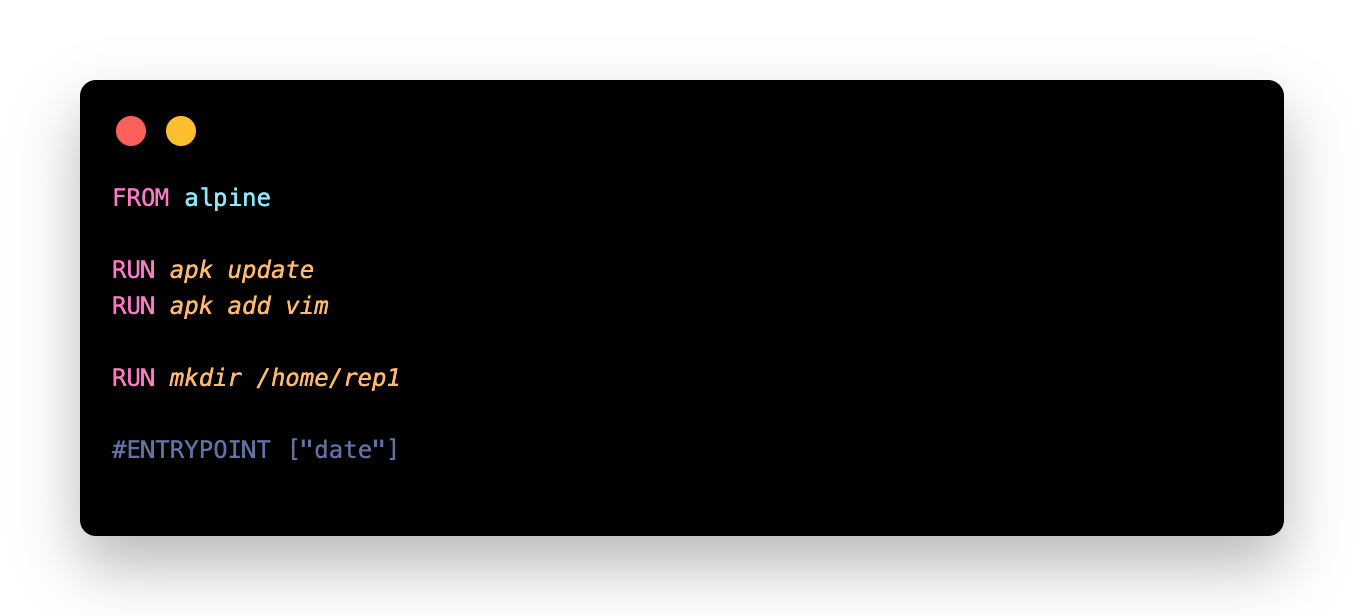
\includegraphics[width=1\textwidth]{img/code1.png}
    \caption{Dockerfile}
    \label{fig:dockerfile}
\end{figure}

\newpage
\subsubsection{Question c}
J'ai donc refait exactement les mêmes commandes que précédemment pour compiler
ce nouveau fichier, et le lancer avec \textbf{docker run -it afficher-date}.
Une fois dans le conteneur je peux vérifier que le dossier a bien été crée et 
qu'il contient bien l'éditeur vim :
\begin{figure}[h]
    \centering
    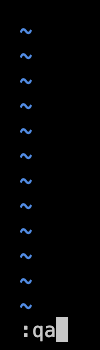
\includegraphics[width=0.1\textwidth]{img/vim.png}
    \caption{vim}
    \label{fig:vim}
\end{figure}
\begin{figure}[h]
    \centering
    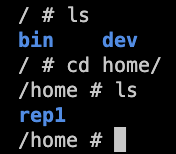
\includegraphics[width=0.2\textwidth]{img/rep.png}
    \caption{Répertoire}
    \label{fig:rep}
\end{figure}
\subsection{Dockerfile - un peu plus loin}
\subsubsection{Question a}
\textbf{docker build -t mydockerfile -f mydockerfile .}

\subsubsection{Question b}
\textbf{docker run -it mydockerfile}

\newpage
\subsubsection{Question c}
Voici donc le script utilisé pour créer le conteneur :

\begin{figure}[h]
    \centering
    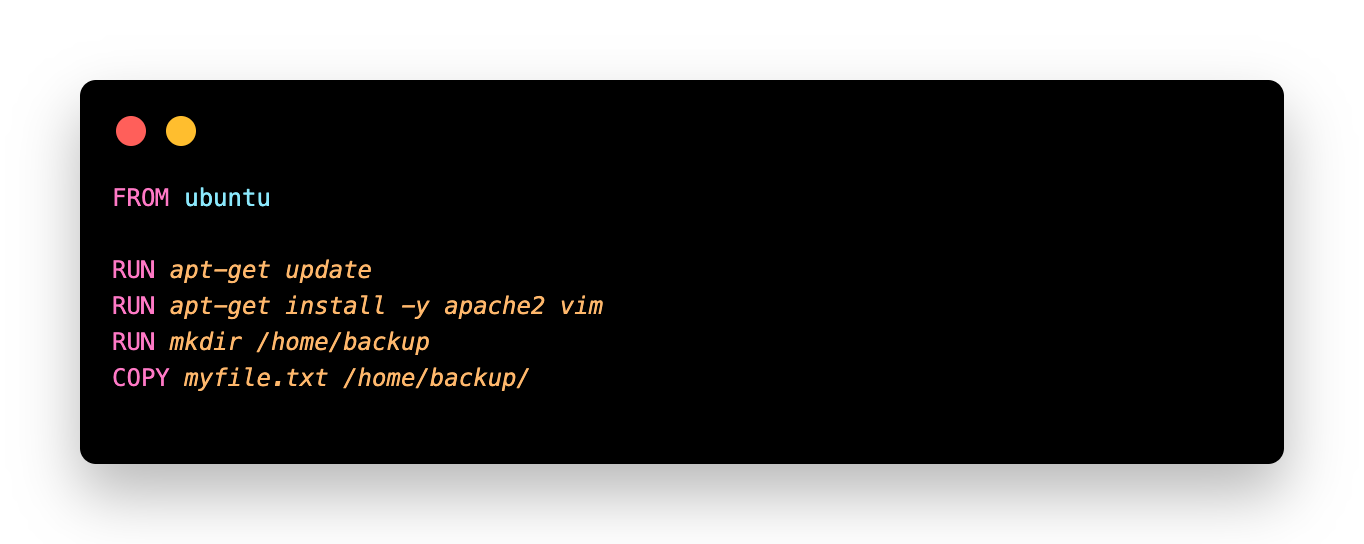
\includegraphics[width=1\textwidth]{img/code2.png}
    \caption{Conteneur 2}
    \label{fig:cont}
\end{figure}
Et donc je peux aller dans le conteneur pour vérifier la présence du fichier.
Je peux aussi bien évidemment écrire dedans.
\begin{figure}[h]
    \centering
    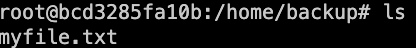
\includegraphics[width=0.8\textwidth]{img/vim1.png}
    \caption{ls}
    \label{fig:vim1}
\end{figure}
\begin{figure}[h]
    \centering
    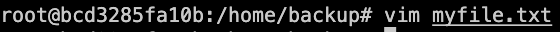
\includegraphics[width=0.8\textwidth]{img/vim2.png}
    \caption{vim myfile.txt}
    \label{fig:con1t}
\end{figure}
\subsubsection{Question d}
J'ai donc arrêté le docker et je me suis rendu compte que les modifications
ne sont pas persistantes. Pour faire ceci, il faut utiliser un volume, avec la commande
suivante : \textbf{docker run -it -v /Users/martinbaumgaertner/R4ROM19-outils-devops/TP2/mydockerfile:/home/backup mydockerfile}
\newpage
\subsection{Publier son image sur un registry privé}
\subsubsection{Question a-b-c}
J'ai donc crée un dockerile avec uniquement \textbf{FROM alpine}. Ensuite, j'ai crée
l'image du dockerfile avec la commande suivante, en précisant comme tag mon 
prénom :
\textbf{docker build -t martinbaumg/martin-baumgaertner:martin -f /Users/martinbaumgaertner/R4ROM19-outils-devops/TP2/docker/dockerfile .}\\

Puis, avec \textbf{1.0} : 
\textbf{docker build -t martinbaumg/martin-baumgaertner:1.0 -f /Users/martinbaumgaertner/R4ROM19-outils-devops/TP2/docker/dockerfile .}

\subsubsection{Question d-e}
J'ai donc mis le docker en ligne avec la commande suivante :\\
\textbf{docker push --all-tags martinbaumg/martin-baumgaertner}\\

Et je vérifie que l'image est bien présente sur dockerhub ce qui est bien le cas,
comme le démontre la capture d'écran suivante :

\begin{figure}[h]
    \centering
    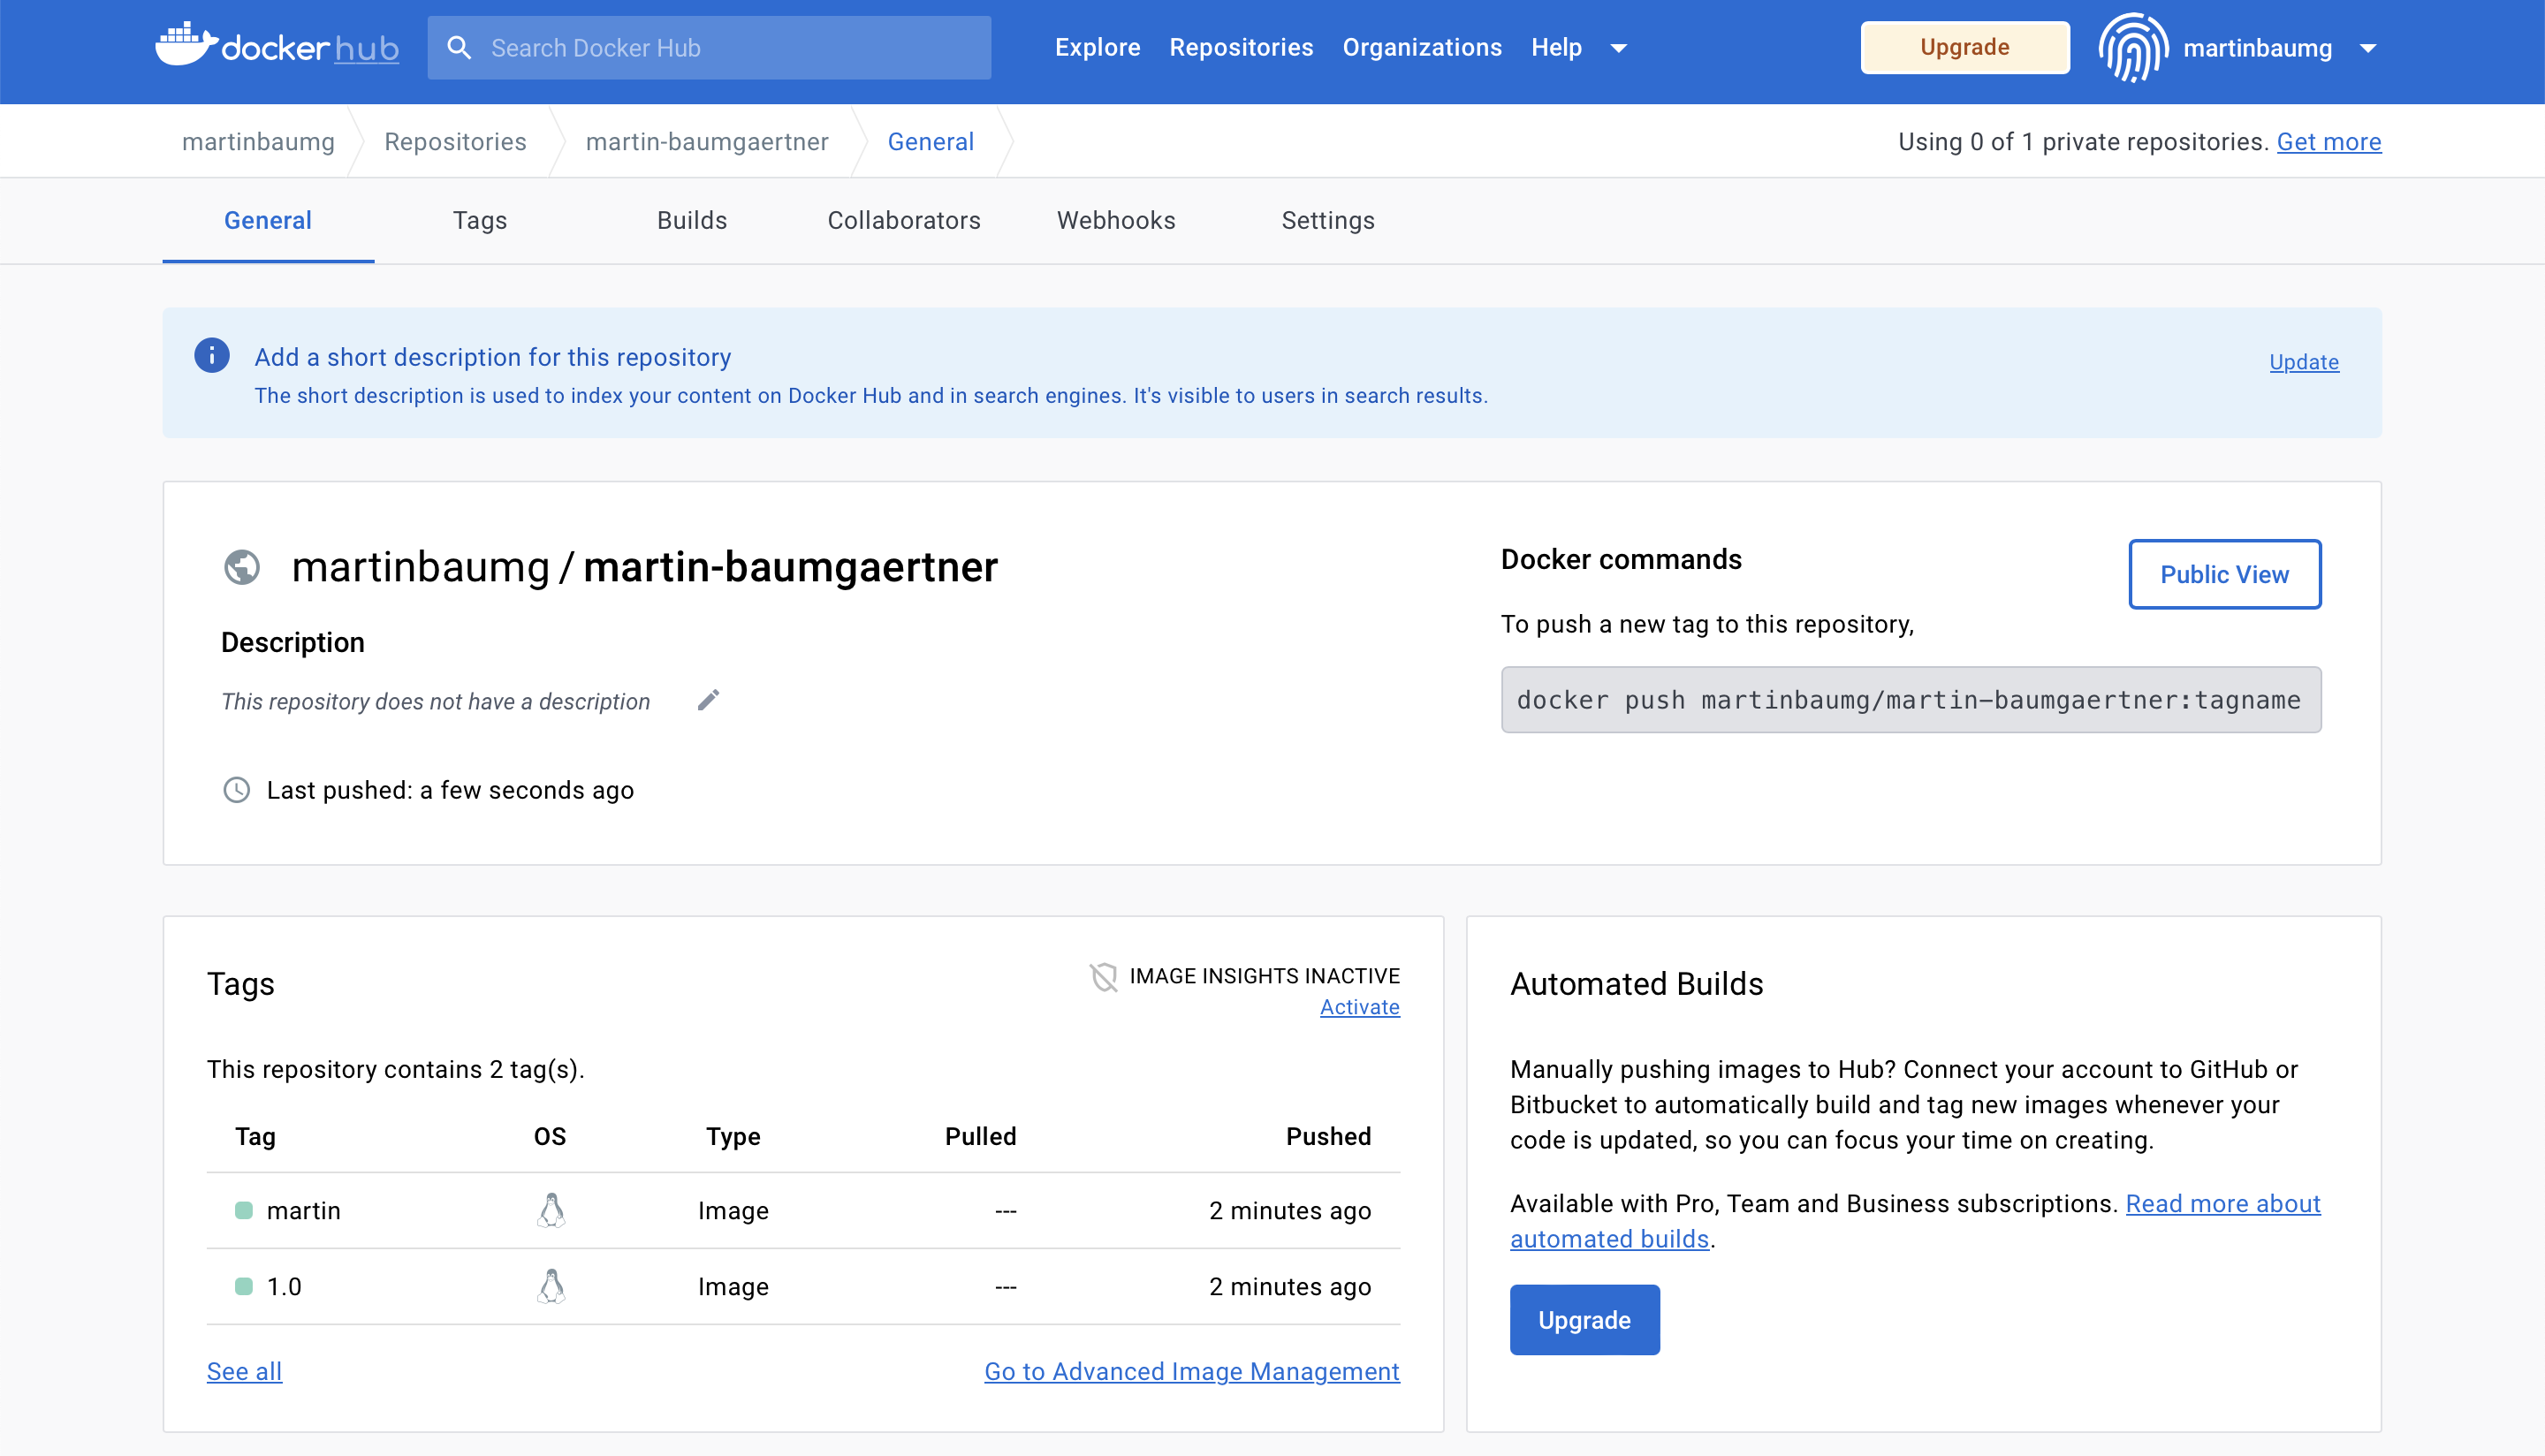
\includegraphics[width=0.8\textwidth]{img/docker-hub.png}
    \caption{dockerhub}
    \label{fig:docker}
\end{figure}

\newpage
\section{Script bash pour créer et éxecuter un conteneur Docker}
J'ai donc crée le script comme demandé. que vous pourrez trouver après ces 
quelques lignes d'explications. Premièrement je lance bien le script
avec la commande \textbf{sh run\_flask.sh}. Je peux ensuite vérifier que l'ID
est le même qui s'affiche dans la console quand je me connecte au conteneur en 
mode interfactif : 
\begin{figure}[h]
    \centering
    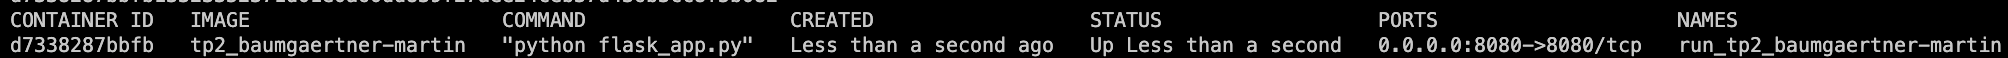
\includegraphics[width=1\textwidth]{img/id1.png}
    \caption{ID}
    \label{fig:id1}
\end{figure}
\begin{figure}[h]
    \centering
    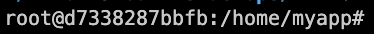
\includegraphics[width=1\textwidth]{img/id2.png}
    \caption{nom dans le conteneur}
    \label{fig:id2}
\end{figure}
Lorsque je démarre le conteneur en mode interfactif avec la commande 
\textbf{docker exec -it run\_tp2\_baumgaertner-martin /bin/bash} et que je 
me connecte depuis un nagicateur web, j'arrive bien sur la page suivante :
\begin{figure}[h]
    \centering
    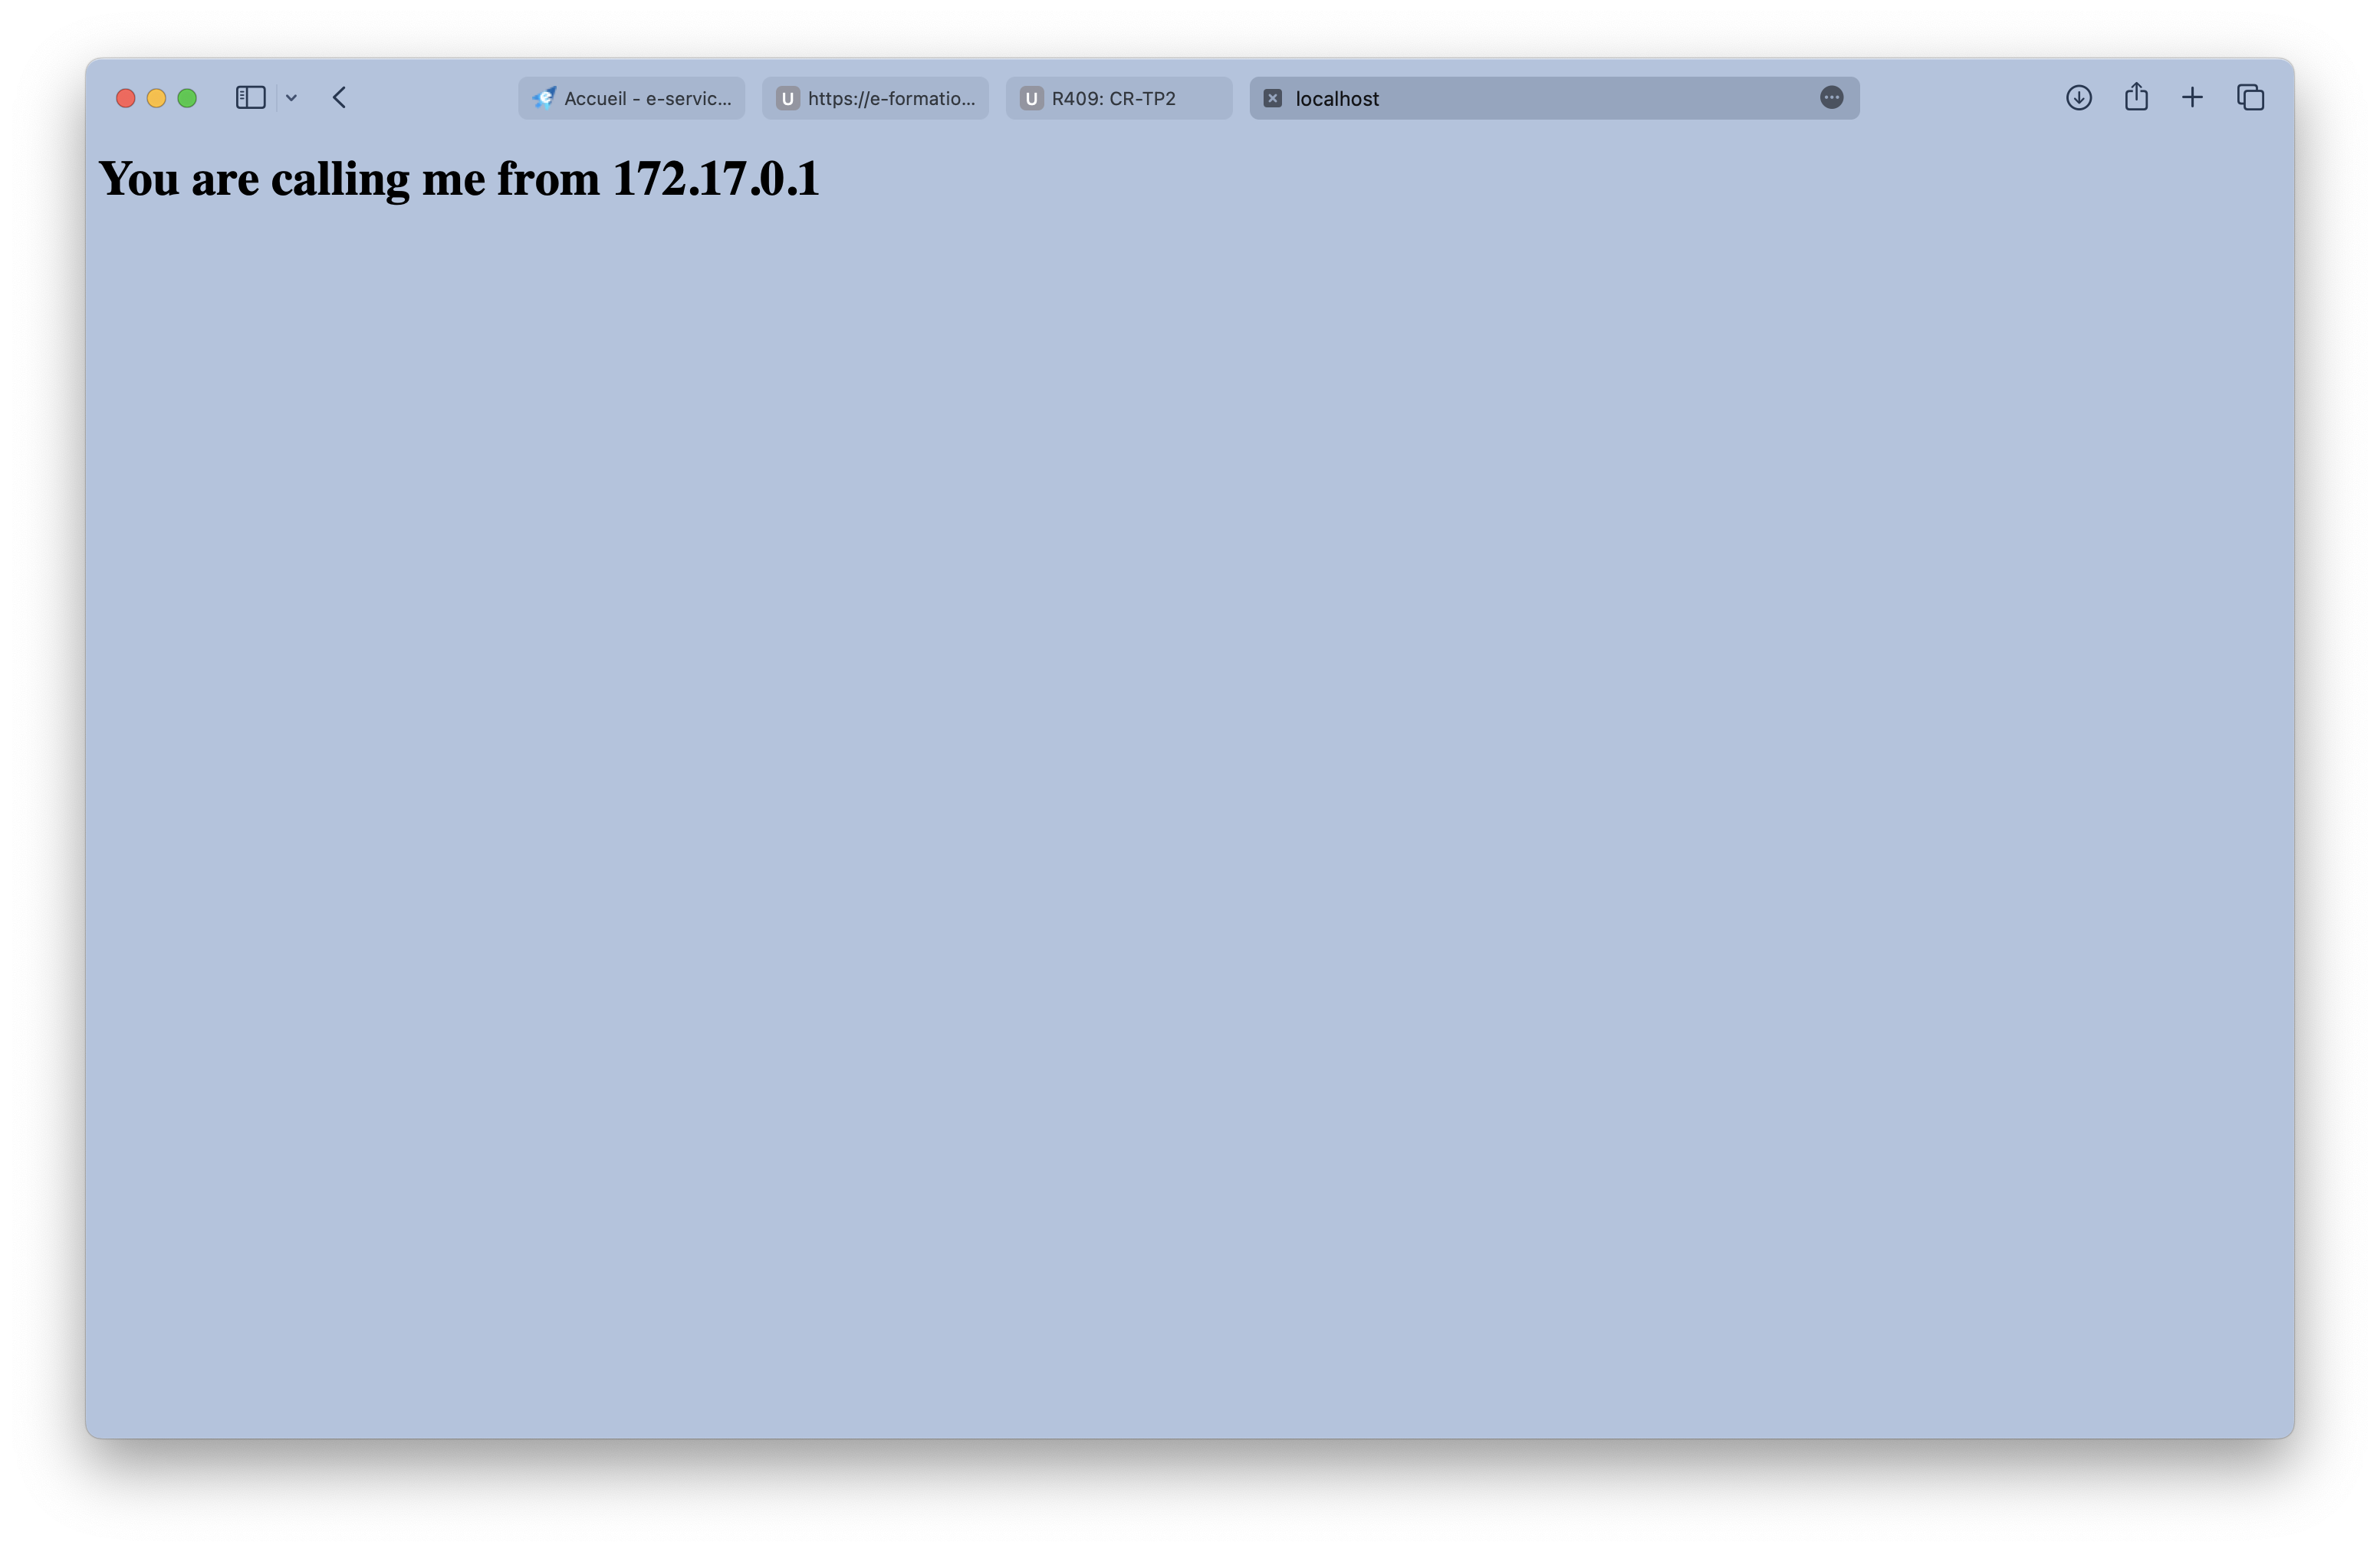
\includegraphics[width=0.8\textwidth]{img/page.png}
    \caption{page flask}
    \label{fig:page}
\end{figure}

\newpage
\subsection{Le script}
Voici le script qui a été utilisé : 
\begin{figure}[h]
    \centering
    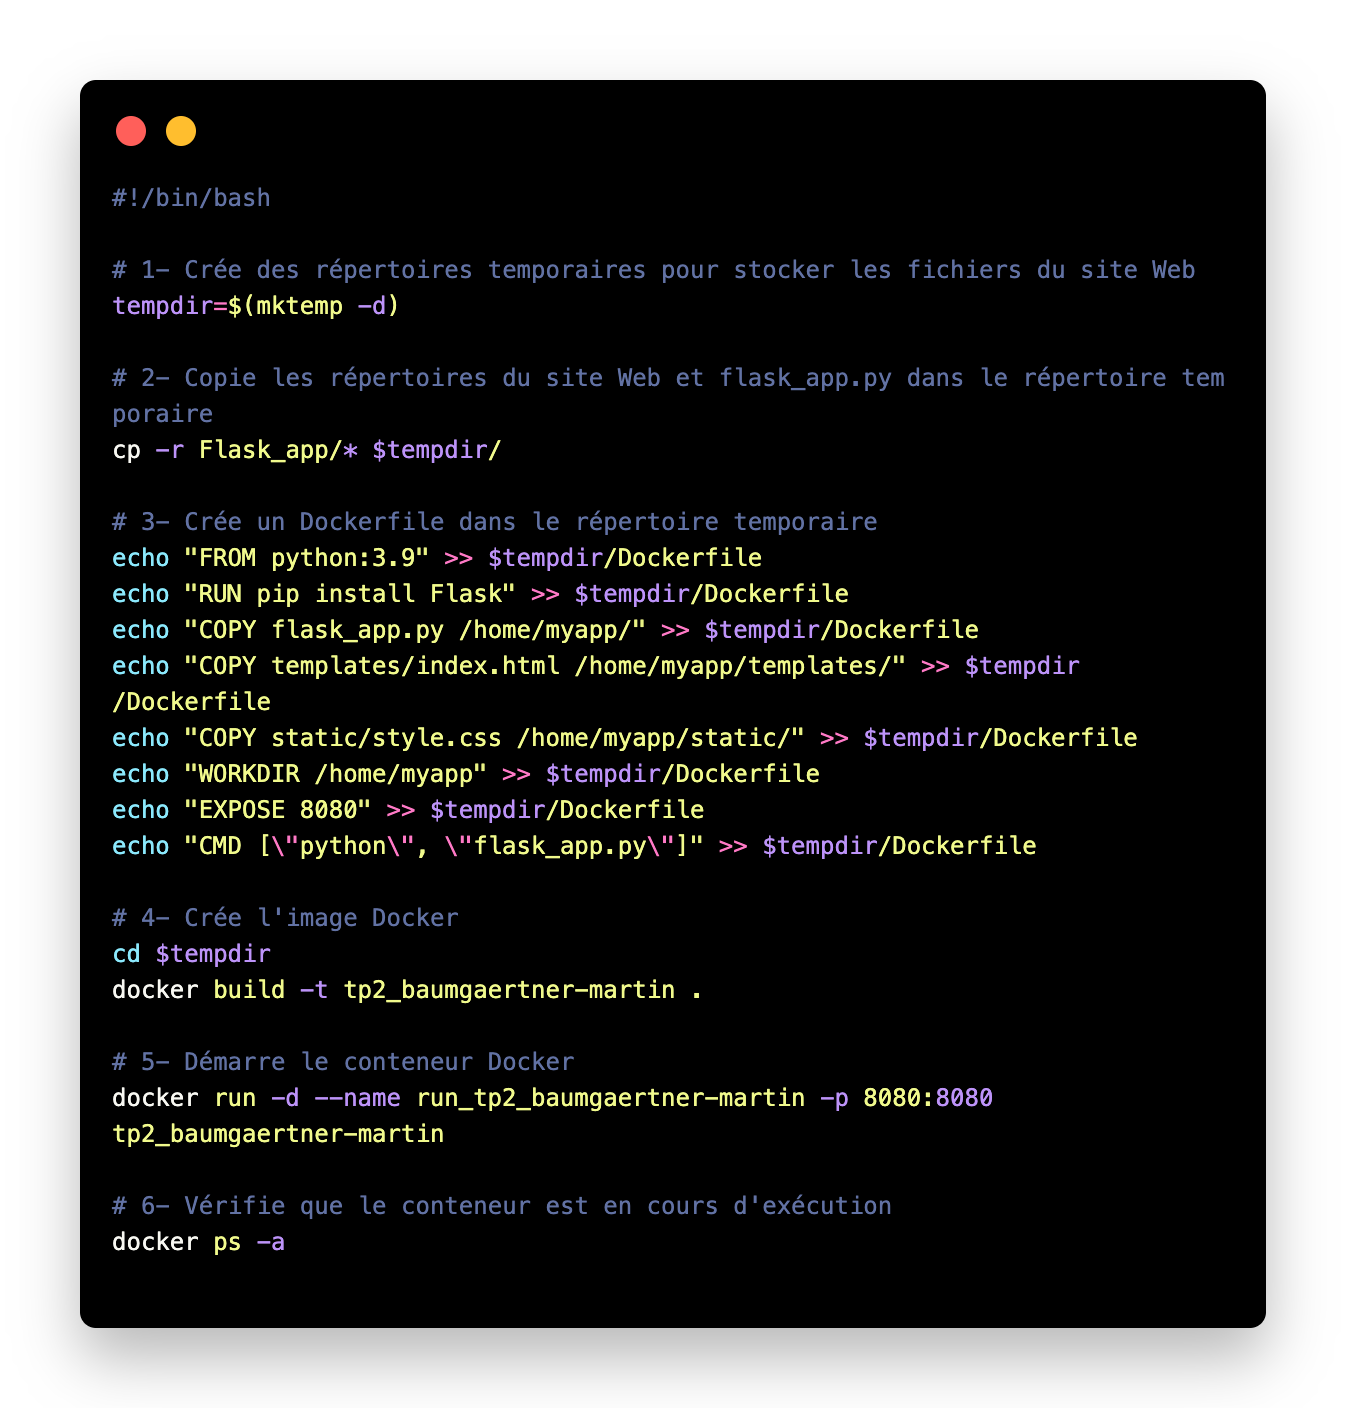
\includegraphics[width=0.9\textwidth]{img/script-f.png}
    \caption{script final}
    \label{fig:script-final}
\end{figure}

\end{document}